\documentclass[crop,tikz,convert={outext=.svg,command=\unexpanded{pdf2svg \infile\space\outfile}},multi=false]{standalone}

\usepackage{amsmath}
\usepackage{amssymb}
\usepackage{mathtools}
\usepackage{fullpage}
\usepackage[T1]{fontenc}
\usepackage{lmodern}
\usepackage{tikz}
\usetikzlibrary{calc,intersections,through,backgrounds}
\usetikzlibrary{bayesnet}
\usepackage{tikzscale}
\usepackage{tkz-euclide}
\usepackage{tcolorbox}
\tcbuselibrary{skins,breakable}
% pgfplots
\usepackage{pgfplots}
\pgfplotsset{compat=1.8}
% For entities in pgfplots
\newcommand{\entpgf}[1]{\texttt{#1}}

\begin{document}
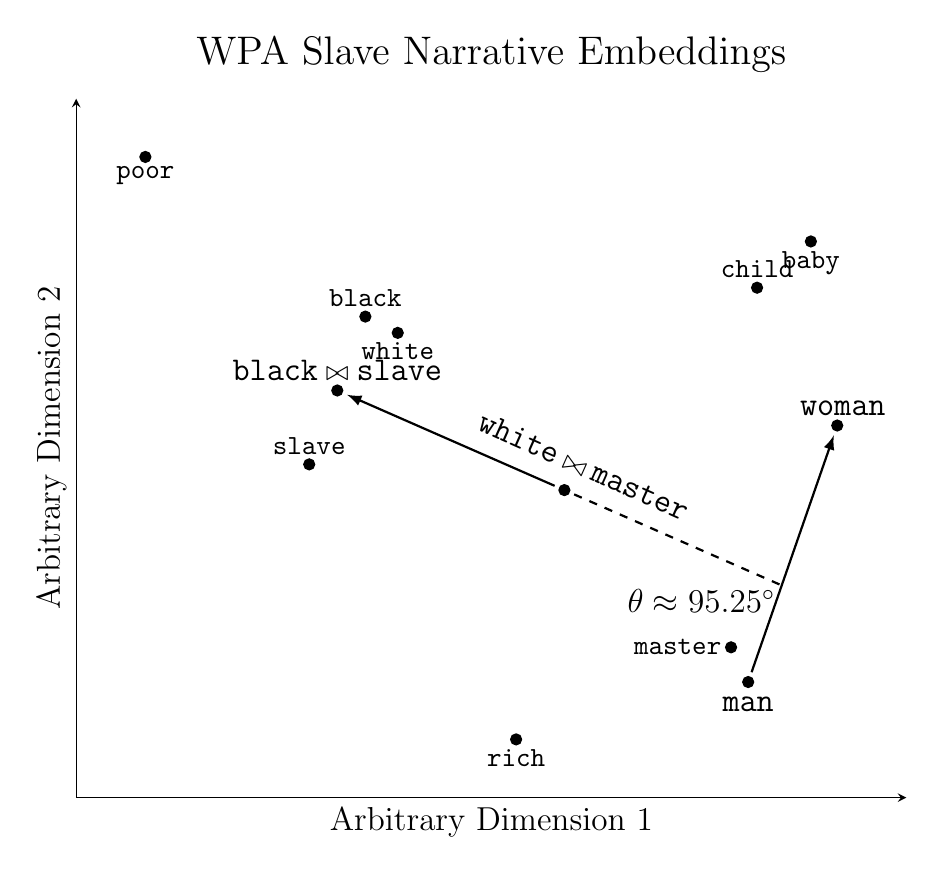
\begin{tikzpicture}
\pgfplotsset{ticks=none}
		\begin{axis}[
			title={\Large WPA Slave Narrative Embeddings},
		    axis x line=bottom,
			axis y line=left,
			xmin=34.371693-1.7909069061279297, xmax=52.28076+1.7909069061279297,
			ymin=8.950363-1.1716894149780275, ymax=20.667257+1.1716894149780275,
			xtick={34.371693,52.28076},ytick={8.950363,20.667257},
			xlabel={\large Arbitrary Dimension 1},ylabel={\large Arbitrary Dimension 2},
			%x label style={anchor=west},
			%y label style={anchor=south},
			width=\textwidth
			]
			\addplot+[mark options={fill=black,color=black},only marks,point meta=explicit symbolic, nodes near coords] coordinates {
(49.975616455078125, 10.104655265808105)[]
(52.28076171875, 15.264684677124023)[]
(49.532535552978516, 10.802817344665527)[]
(40.06618118286133, 17.45557975769043)[]
(38.61276626586914, 14.48298168182373)[]
(40.904022216796875, 17.128196716308594)[]
(50.20615768432617, 18.036758422851562)[]
(51.59844207763672, 18.967124938964844)[]
(34.3716926574707, 20.66725730895996)[]
(43.968379974365234, 8.950363159179688)[]
(45.21827697753906, 13.965507507324219)[]
(39.339473724365234, 15.969280242919922)[]

};
\node (man) at (axis cs:49.975616, 10.104655){};
\node (woman) at (axis cs:52.28076, 15.264685){};
\node (master) at (axis cs:49.532536, 10.802817){};
\node (black) at (axis cs:40.06618, 17.45558){};
\node (slave) at (axis cs:38.612766, 14.482982){};
\node (white) at (axis cs:40.904022, 17.128197){};
\node (child) at (axis cs:50.206158, 18.036758){};
\node (baby) at (axis cs:51.598442, 18.967125){};
\node (poor) at (axis cs:34.371693, 20.667257){};
\node (rich) at (axis cs:43.96838, 8.950363){};
\node (whitemaster) at (axis cs:45.218277, 13.9655075){};
\node (blackslave) at (axis cs:39.339474, 15.96928){};
\node [inner sep=0] (intersect) at (axis cs:50.8438, 12.048069){};
\node[anchor = north, xshift=0.0, yshift=-2.0] (manl) at(axis cs: 49.975616, 10.104655){${\large \entpgf{man}}$};
\node[anchor = south, xshift=2.0, yshift=0.0] (womanl) at(axis cs: 52.28076, 15.264685){${\large \entpgf{woman}}$};
\node[anchor = east, xshift=0.0, yshift=0.0] (masterl) at(axis cs: 49.532536, 10.802817){$\entpgf{master}$};
\node[anchor = south, xshift=0.0, yshift=0.0] (blackl) at(axis cs: 40.06618, 17.45558){$\entpgf{black}$};
\node[anchor = south, xshift=0.0, yshift=0.0] (slavel) at(axis cs: 38.612766, 14.482982){$\entpgf{slave}$};
\node[anchor = north, xshift=0.0, yshift=0.0] (whitel) at(axis cs: 40.904022, 17.128197){$\entpgf{white}$};
\node[anchor = south, xshift=0.0, yshift=0.0] (childl) at(axis cs: 50.206158, 18.036758){$\entpgf{child}$};
\node[anchor = north, xshift=0.0, yshift=0.0] (babyl) at(axis cs: 51.598442, 18.967125){$\entpgf{baby}$};
\node[anchor = north, xshift=0.0, yshift=0.0] (poorl) at(axis cs: 34.371693, 20.667257){$\entpgf{poor}$};
\node[anchor = north, xshift=0.0, yshift=0.0] (richl) at(axis cs: 43.96838, 8.950363){$\entpgf{rich}$};
\node[anchor = south, xshift=4.0, yshift=2.0,rotate=-24] (whitemasterl) at(axis cs: 45.218277, 13.9655075){${\large \entpgf{white} \bowtie \entpgf{master}}$};
\node[anchor = south, xshift=0.0, yshift=0.0] (blackslavel) at(axis cs: 39.339474, 15.96928){${\large \entpgf{black} \bowtie \entpgf{slave}}$};
\node[anchor = north, xshift=-29.0, yshift=2.0] (intersectl) at(axis cs: 50.8438, 12.048069){\large $\theta \approx 95.25^\circ$};
\draw[->,>=stealth,thick,,-latex](man) to (woman);
\draw[->,>=stealth,thick,,-latex](whitemaster) to (blackslave);
\draw[-,dashed,>=stealth,thick,](whitemaster) to (intersect);

\end{axis}
\end{tikzpicture}
\end{document}